\chapter[Classification]{Classification}
\label{ch:classification}
\index{classification|(}

% Data mining can be described as ''the procedure of extracting information from huge sets of data''. 
Classification and regression\index{Regression} are two techniques which are nowadays being used to extract knowledge and perform predictions on the huge amounts of available data \citep{sagar2017}. These techniques predict values which may be either \textit{quantitative}\index{classification!quantitative predictions} - involving discrete numerical values, or \textit{qualitative}\index{classification!qualitative predictions} - with values within a particular class or label \citep{james2006}. Predicting marks that students will obtain in their final exams yields a discrete, continuous value. In this case, regression analysis is ''used to predict missing or unavailable numerical data values'' \citep{jiawei2011}. On the other hand, predicting the grade (A, B or C) that the students will obtain is considered as a classification problem, since the outcome value is a categorical class label \citep{jiawei2011}.\\

Classification is a data analysis technique in which models, also referred to as \textit{classifiers}\index{classification!classifiers}, are used to ''predict categorical (discrete, unordered) class labels''. Several scenarios in the real world may require classification models to predict several outcomes. For example, in the health sector, classification can be helpful in predicting whether a person is diagnosed with a particular medical condition or not, based on certain parameters related to experienced symptoms \citep{venkata2011,alzahani2015}. Financial sectors may find classifications helpful when it comes to predicting whether a company is bankrupt or in good financial health \citep{moradi2012}. Moreover, they may apply classifiers to determine whether a bank should issue a loan to a customer \citep{thomas2000}. In these scenarios, classifiers predict labels such as 'positive' or 'negative' for a medical condition, or 'bankrupt' or 'healthy' for the financial status of a company. Since values predicted by a classifier are discrete, any ordering amongst the values is meaningless. 

Classification involves two main steps: training a model for classification, and then using the model to classify the data. When \textit{supervised learning}\index{classification!supervised learning} is used for classification, the training stage involves analysing a training data consisting of samples which are labelled with a categorical class. These samples are used to train the model on how to perform classifications. Testing data, also made up of features and their corresponding class labels, is then used to predict the accuracy of the classifier, by comparing the predicted outcome to the actual class label in the testing samples \citep{neelamegam2013}. On the other hand, \textit{unsupervised learning}\index{classification!unsupervised learning} builds classifiers for predictions using data which is unlabelled, i.e.\ the final class is not known. In this case, the model learns how to classify the data by observing the similarities or dissimilarities within the dataset \citep{jiawei2011}.

\section{Binary Classification}
\label{sec:binary classification}
\index{classification!binary classification}


When two classes are available as outputs of a classification problem, then this is called binary classification \citep{neelamegam2013}. \citet{kolo2011} defines \textit{binary classifiers}\index{classification!binary classification!binary classifiers} as those which determine whether an input should classify as ''either in the category or not in the category''. This implies that an input which classifies as not part of a class should automatically be considered as a member of the other class. \begin{marginfigure}
    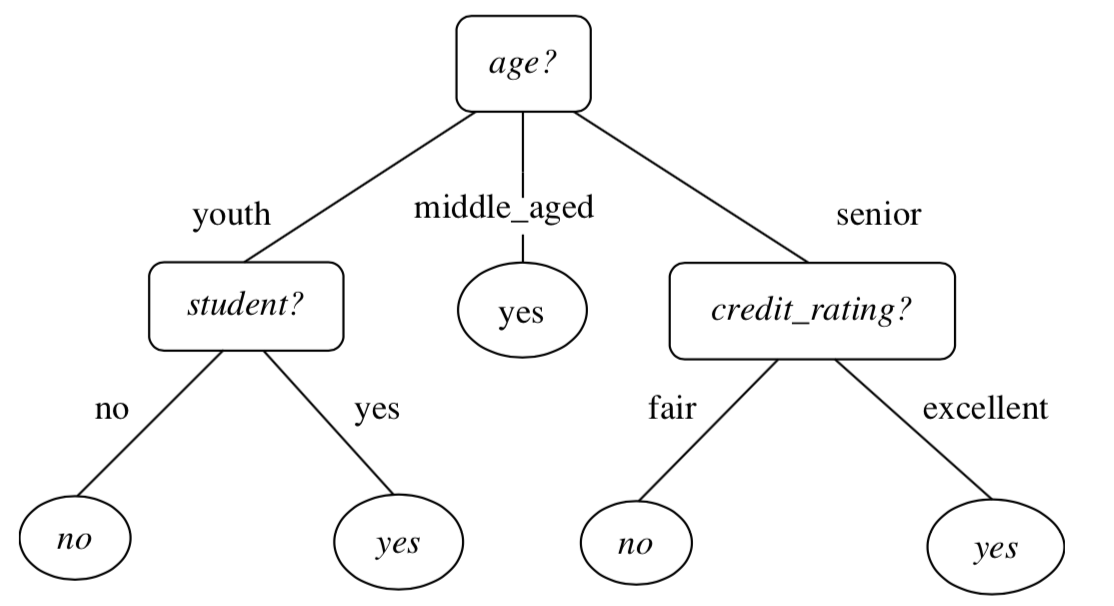
\includegraphics{graphics/classification/BinaryDecisionTree.png}
    \caption{
    A binary Decision Tree example which determines whether a customer will purchase a computer or not. 
    Reproduced from \citet{jiawei2011}.
    }
    \label{fig:binary-decision-tree}
\end{marginfigure}
For example,  using a binary classifier to predict 'Pass' or 'Fail' in a subject, by providing it with the marks obtained in the exam, the classifier should determine whether the student 'passed' or 'did not pass' an exam. A 'Fail' label is assumed when the classifier determines that the student 'did not pass' the exam \citep{kolo2011}. Decision Trees (Figure~\ref{fig:binary-decision-tree}), Bayesian Networks and Logistic Regression are some of the methods used for binary classification.  

\section{Probabilistic Classification}
\label{sec:probabilistic classification}
\index{classification!probabilistic classification} 
Probabilistic classification can be considered as a subclass of classification, in which apart from assigning categorical classes to unseen data, probabilistic models ''use statistical inference to find the best class for a given example'' \citep{aggarwal2014}. This implies that probabilistic models compute the probability that an unseen example belongs to the possible target classes, and then chooses the final target class by considering the highest probability obtained. One advantage of probabilistic models is that the prediction outcome is composed of both the target label, as well as the confidence with which this class label was obtained. 

Initially, probabilistic classification involves the estimation of the posterior probability, P($C_k$|$x$), where $C_k$ denotes the class and $x$ refers to the input variables. This posterior probability estimate can be determined using a \textit{generative model}\index{classification!probabilistic classification!generative model} or a \textit{discriminative model}\index{classification!probabilistic classification!discriminative model}. Generative models work by obtaining the probability of each class, denoted by P($C_k$), as well as the probability of obtaining $x$ when given a class, also known as the class-conditional probabilities, denoted by P($x$|$C_k$) \citep{aggarwal2014}. Then, the posterior probability can be determined using Bayes Theorem, shown in Equation~\ref{eq:bayesTheorem1}, or by modelling the joint distribution over $x$ and $C_k$ as in Equation~\ref{eq:jointDistribution}. 
\begin{equation}
    \label{eq:bayesTheorem1}
    P(C_k|x) = P(C_k)\cdot\frac{P(x|C_k)}{P(x)}
\end{equation}

\begin{equation}
    \label{eq:jointDistribution}
    P({C_k}|x) \propto P(C_k)\cdot P(x|C_k)
\end{equation}
\pagebreak[1]

In these equations $C_k$ denotes the class and $x$ refers to the input variables. Hidden Markov Model and Naive Bayes classifier are two examples of generative models used in probabilistic classification. Discriminative models focus on determining a function that maps the input $x$ directly onto the class $C_k$. 

\begin{equation}
    \label{eq:logisticRegression}
    P(C_k|x) = \frac{1}{1+e^{-\theta^{T}X}}
\end{equation}

One popular discriminative model is the Logistic Regression Model, explained by Equation~\ref{eq:logisticRegression}, in which $\theta$ refers to the parameters to be estimated. Conditional Random Fields is another commonly used discriminative model. 

Once the posterior probability is obtained, probabilistic classification then uses decision theory to deduce the class of an unseen example $x$ \citep{aggarwal2014}. 

\section{Multiclass Classification}
\label{sec:multiclass}
\index{classification!multiclass classification}

Multiclass classification models are able to determine a class for an unseen example from $k$ classes, where $k$ > 2. A multiclass classification problem may be solved by extending the aforementioned binary classification algorithms, and others including \textit{Neural Networks}\index{classification!multiclass classification!neural networks} and \textit{Support Vector Machines}\index{classification!multiclass classification!support vector machines} \citep{aly2005}. For example, a Decision Tree algorithm can naturally handle multiclass classification problems. To predict an outcome using the tree model, the algorithm starts from the root node of the tree and repeatedly traverses branches based on the feature values, until a leaf node is reached \citep{rokach2014}. The value of the leaf node is considered as the predicted class label of the unseen example, and these values can refer to any of the $k$ classes. Support Vector Machines are another example of classification algorithms which were initially built for binary classification, but eventually extended to be applied in multiclass problems. Extensions of this algorithm handle the separation of the various classes by amending the optimization problem \citep{aly2005}.   

\citet{aly2005} discusses approaching a multiclass classification problem by decomposing it into multiple binary classification problems, which can then be solved using binary classifiers.

\subsection{One-versus-all (OVA)} \index{classification!multiclass classification!one-versus-all}
This approach considers $k$ binary classifiers, where $k$ is the number of classes. Each classifier is trained on data composed of positive examples from the $k^{th}$ class and negative examples from the remaining $k$-1 classes. Unseen examples are assigned the class of the classifier which obtains the highest output \citep{aly2005}.

\subsection{All-versus-all (AVA)} \index{classification!multiclass classification!all-vs-all}

In this approach, $\frac{k(k-1)}{2}$ binary classifiers are built to distinguish between all the possible pairs of classes. When predicting, all classifiers are considered and the class obtaining the highest score is taken as the target class \citep{aly2005}.

\subsection{Error-Correcting Output-Coding (ECOC)}\index{classification!multiclass classification!error-correcting output-coding} 
Using this approach for multiclass classification, $n$ binary classifiers are trained to differentiate between $K$ classes. A binary matrix $M$ (Figure~\ref{fig:classification-ecoc}) is composed of $K$ classes and the corresponding codewords with length $N$. Thus, binary classifiers are trained using the column values of $M$.
\begin{marginfigure}
    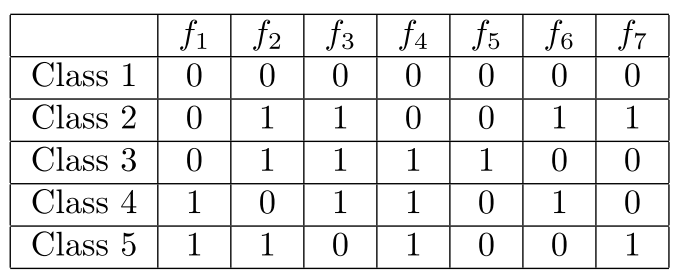
\includegraphics{graphics/classification/ECOC.png}
    \caption{
    ECOC Binary Matrix. 
    Reproduced from \citet{aly2005}.
    }
    \label{fig:classification-ecoc}
\end{marginfigure} 
When predicting labels for unseen examples, a distance measure is used to compare codewords obtained from the $N$ classifiers to the $K$ codewords. The class label is determined by selecting the codeword having the smallest distance \citep{aly2005}. \\


Apart from these methods, \textit{Generalized Coding}\index{classification!multiclass classification!generalized coding} \citep{allwein2001} may also be applied. Finally, multiclass classification problems may be handled using \textit{hierarchical classification}\index{classification!multiclass classification!hierarchical classification}, in which classes are arranged in the form of a tree. Parent nodes of the trees are further split into child nodes, and a binary classifier is used to differentiate between the clusters pertaining to child classes. Eventually, the leaf node constitutes of a single class, thus the model can then be used to classify a new example \citep{aly2005}. Binary Hierarchical Classifier (BHS) \citep{kumar2002} and Hierarchical SVM (HSVM) \citep{yangchi2014} are two hierarchical classification approaches. 

\index{classification|)}